\section{The positive quotient and the actual supported Gysin
receiver}\label{the-positive-quotient-and-the-actual-supported-gysin-receiver}

The complete received RGR proof constructs the actual continuous-current
Gysin receiver from the original source, its signed differential, both
endpoint lines, its dual original extension and the separate
positive-adjoint obstruction. The next GDC proof calculates its complete
strong-dual image, raw and separated costalk quotients, and the
canonical maps to the already constructed positive receiver.

The original source appears again as an explicit restricted Fréchet
extension. Its transpose is the actual separated costalk row, with
topological inverses proved through compactness and Hahn--Banach. A
continuous-current quotient kills the exact closed defect image; its
full coefficient kernel remains in a proved triangle. All nontrivial
positive coefficient scales have the same unclosed image and isomorphic
receivers, with explicit bounded inverses and a cocycle law.

\begin{figure}
\centering
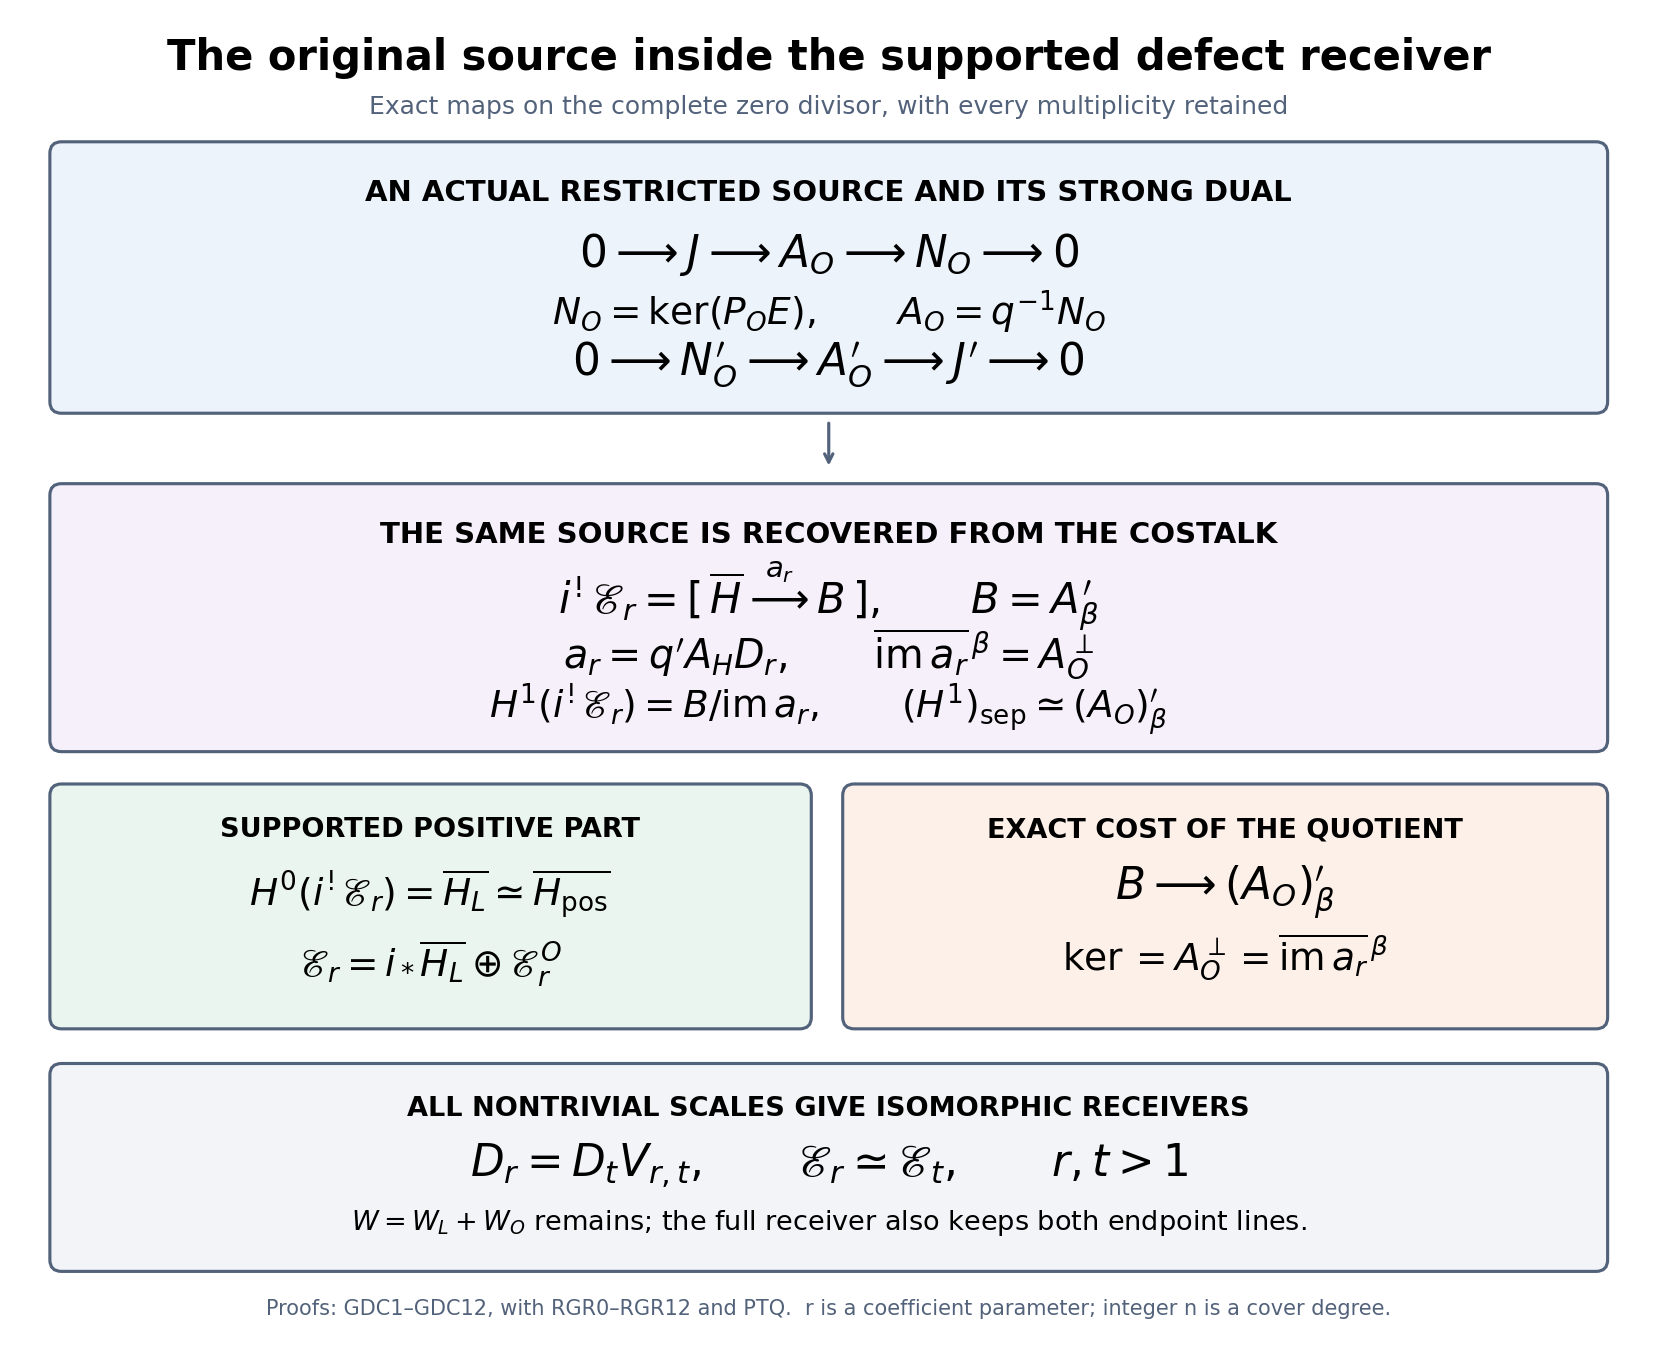
\includegraphics[width=0.9\linewidth,height=\textheight,keepaspectratio,alt={Exact source and supported-cohomology comparison. Here N\_O is the source whose off-line values vanish, A\_O is its inverse image in the original A, and B is the strong dual of A. The reduced receiver retains its raw degree-one quotient and its separated comparison; the full receiver additionally retains both labelled endpoint lines by GDC4.7. The lower-left summand is the conjugate universal positive quotient. The original Weil form retains both terms. Complete proofs: GDC1--GDC12 and received RGR0--RGR12; the positive universal property is PTQ3--PTQ4.}]{gysin_positive_receiver.png}
\caption{Exact source and supported-cohomology comparison. Here N\_O is
the source whose off-line values vanish, A\_O is its inverse image in
the original A, and B is the strong dual of A. The reduced receiver
retains its raw degree-one quotient and its separated comparison; the
full receiver additionally retains both labelled endpoint lines by
GDC4.7. The lower-left summand is the conjugate universal positive
quotient. The original Weil form retains both terms. Complete proofs:
GDC1--GDC12 and received RGR0--RGR12; the positive universal property is
PTQ3--PTQ4.}
\end{figure}

The full proofs follow. The final GDC text has complete root
verification, with independent constituent derivations of the scale and
topology comparisons; a complete independent final-text audit is not
claimed. The complete original lifting and arithmetic weight-separation
target remains active. The receiving quotient has a proved kernel; its
existence does not itself make the original defect vanish.
